\chapter{Automatic Optical Inspection}

\section{Ispezione dei dispositivi elettronici}
Nuovi sviluppi nell’assemblaggio di PCB non possono avvenire se non con cambiamenti corrispondenti
nella tecnologia di controllo della qualità \cite{4459975}.
Il test in-circuit è stato per anni il mezzo principale per la rilevazione e la diagnosi dei difetti poichè
rimuovendo la barriera del “design for testability” (La realizzazione di un progetto introducendo parti e
componenti accessorie volte a facilitare o a permettere test altrimenti impossibili) ha reso possibile
realizzare sistemi complessi senza la paura di non poterli testare. Il test in circuit è stato per tanto un
approccio semplice ed universale al problema del controllo qualità nell’industria elettronica ma risulta
essere sempre più difficile applicarlo a causa della miniaturizzazione che rende spesso impraticabile il test
tradizionale per mezzo di sistemi a sonde mobili o a letto d’aghi.
Considerando altre tecnologie quale il boundary scan, l’ispezione a raggi x, l’ispezione ottica manuale e
l’ispezione ottica automatica nessuna è in grado di sostituire totalmente il test in-circuit ma è in grado di
complementarlo efficientemente.
Tutti i processi usano l’ispezione ottica manuale. Gli ispettori in uno stabilimento di assemblaggio ben
gestito spesso sprecano la maggior parte del loro tempo ispezionando prodotti non difettosi e usano solo
una frazione del loro tempo in maniera proficua al miglioramento ed al controllo della qualità (ovvero
quando un difetto si presenta loro) esiste un modo tramite cui possiamo focalizzare la potenza dell’occhio
umano solo sui difetti?
Se un sistema AOI è utilizzato per coadiuvare l’ispezione manuale il numero di ispettori decresce (la
semplicità del processo cresce) e la consistenza dell’ispezione migliora. Consideriamo una scheda dove
5000 saldature di cui solo 10 sono inadeguate, se una macchina AOI la ispezionasse prima dell’uomo ed
approvasse tutte le saldature corrette rimarrebbe solo da verificare manualmente le 10 saldature riportate
come critiche dal sistema automatico, date le ambiguità delle performance umane (dovute a stanchezza e
differenze tra individui diversi) adottare questa metodologia porterebbe ad una maggiore efficienza nel controllo qualità

Un sistema AOI non aggiunge nessuna nuovo concetto allo stabilimento, si limita a automatizzare una
categoria di ispezioni già realizzata manualmente.

\subsection {Principio di funzionamento di un sistema AOI}

Un sitema AOI è in grado di acquisire milioni di pixel in una frazione di secondo, questi dati vengono
utilizzati per l’ispezione visuale e per misure di precisione.
Il sistema AOI scansisce visualmente la superfice della scheda elettronica, la scheda è illuminata da
differenti sorgenti luminose ed osservata da uno scanner o da un numero arbitrario di telecamere ad alta
definizione, ogni produttore di sistemi AOI sviluppa degli algoritmi properietari di ispezione e di tecniche
di illuminazione, ciò si traduce in differenti punti di forza o debolezza a seconda della tipologia di
prodotto ispezionato e delle tecniche impiegate.
Illuminare correttamente la parte è una fase critica per un sistema AOI, esso deve essere in grado di
vedere la parte da ispezionare ma soprattutto le caratteristiche distintive del difetto da individuare, la luce amplifica i dettagli salienti e sopprime dettagli categorizzabili come rumore, ad esempio molti prodotti
riflettono la luce causando aree di intensa illuminazione nell’immagini, ciò potrebbe oscurare i dettagli
ricercati durante l’ispezione.
Il dispositivo di imaging traduce la luce riflessa dalla parte da ispezionare in un immagine elettronica che
verrà successivamente elaborata.
Il cervello di un sistema AOI è il “vision computer”, tale computer analizza l’immagine per estrarre misure,
conteggi di parti, colori o altre features visuali necessari all’ispezione.

\section {Tipologie di ispezione ottica automatica delle schede elettroniche}

\subsection{Presenza di un componente}

\begin{figure}[!ht]
\centering
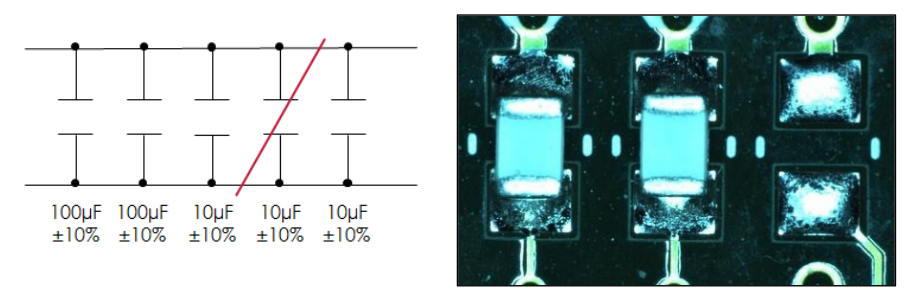
\includegraphics[width=.8\textwidth]{img/presenza-componente.png}
\caption{Test di presenza}
\label{fig:presenza}
\end{figure}

Obiettivo di questo test è verificare la presenza di un componente sulla scheda, ciò assolve al doppio
compito di verifica del componente corretto e controllo dell’assenza di un componente non corretto, i
possibili scenari mitigati sono:
\begin{itemize}
\item Durante un passaggio della catena produttiva costituito da una saldatura manuale l’addetto ha
dimenticato il componente oppure ne ha saldato uno sbagliato;
\item Durante un passaggio della catena produttiva costituito da una posa automatica del componente
e successiva saldatura automatica il sistema pick and place non ha posizionato correttamente il
componente o il processo di saldatura automatica non è stato affidabile provocandone il distacco.
Un test di presenza ottica può completare la copertura dei possibili difetti rimediando a limitazioni del
test in-circuit come l’assenza di un capacità di filtro in parallelo ad altre;
\end{itemize}

\subsection{Posizionamento di un componente}

\begin{figure}[!ht]
\centering
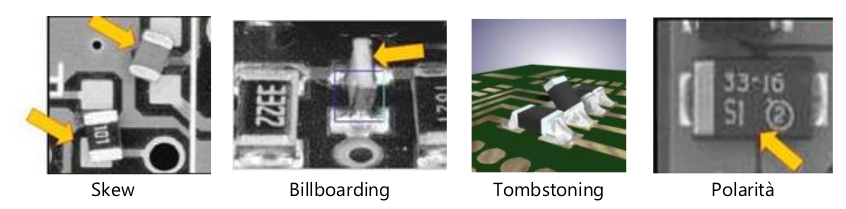
\includegraphics[width=.8\textwidth]{img/vari.png}
\caption{Test di posizionamento}
\label{fig:posizionamento}
\end{figure}.

Obiettivo di questo test è verificare che il montaggio di un componente sia avvenuto correttamente e che
rispetti determinate specifiche meccaniche quali:
\begin{itemize}
\item Skew (rotazione del componente lungo l’asse perpendicolare alla scheda);
\item Offset (traslazione del componente rispetto al baricentro atteso);
\end{itemize}

O che non si siano verificate delle condizioni di posizionamento anomalo:
\begin{itemize}
\item Componente saldato capovolto.;
\item Componente saldato verticalemente sulla scheda. (Billboarding);
\item Componente parzialmente rialzato lungo un lato (Tombstoning);
\item Componente saldato con polarità errata;
\end{itemize}

\subsection{Identificazione di un componente}
Obiettivo di questo test è garantire la tracciabilità delle parti montate su di una scheda o delle schede
testate tramite l’inserimento di un codice nel database del sistema CIM se presente
\begin{description}
\item[Verifica ottica dei caratteri]
La verifica ottica dei caratteri, o OCV, è uno strumento software di elaborazione elettronica delle immagini utilizzato per controllare la qualità di stampa o marcatura di una stringa di riconoscimento ottico dei caratteri (OCR) e confermarne la leggibilità. Oltre a verificare che il contenuto della stringa di testo presentata sia corretto, provvede anche a controllarne la qualità, il contrasto e la nitidezza, segnalando o rifiutando i campioni di scarsa qualità.
Un’applicazione fondamentale che utilizza l’OCV è la verifica dei codici di data e lotto (stampati su un’etichetta o marcati direttamente sulla confezione o sul prodotto) nel confezionamento di prodotti farmaceutici, dispositivi sanitari, cosmetici e altri beni di consumo.
Viene utilizzato un software OCR per leggere una stringa di testo e per provare a leggere anche un testo di scarsa qualità o rovinato, formulando l’ipotesi migliore sui dati. Sarà poi il software OCV a controllare la qualità e confermare la leggibilità del testo. Questo controllo viene attuato molto spesso per confermare che i codici di data e lotto stampati siano corrispondenti a quelli attesi.
\item [Riconoscimento ottico dei caratteri] A differenza della verifica dei caratteri il riconoscimento non parte da una base conosciuta ma viene usato per riconoscere ed interpretare i caratteri impressi su di un dispositivo per poi inserirli in un database o intraprendere azioni differenti.
\item [Lettura di codici a barre] Un codice a barre viene impresso sui dispositivi al fine di rappresentare un mezzo ottico affidabile e compatto per trasportare dei dati facilmente estraibili da sistemi automatici.

\end{description}

\subsection{Test della saldatura}

\begin{figure}[!ht]
\centering
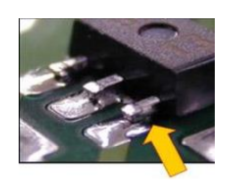
\includegraphics[width=.4\textwidth]{img/saldatura.png}
\caption{Test della saldatura}
\label{fig:presenza}
\end{figure}

Obiettivo di questo test è garantire che il processo di saldatura sia conforme alle specifiche di produzione,
alcuni categorie di difetti rilevabili sono:
\begin{itemize}
\item Pin sollevati/aperti;
\item Cortocircuiti tra i pin dovuti a leghe saldanti in eccesso;
\item Giunti di saldatura con eccesso o insufficienza di lega saldante;
\item Saldatura fredda;
\end{itemize}

\subsection{Test del circuito stampato}
Obiettivo di questo test è garantire che il circuito stampato sia integro prima dell’effettiva popolazione,
alcune categorie di difetti rilevabili sono:
\begin{itemize}
\item Cortocircuiti tra le piste;
\item Piste interrotte;
\item Pad o altre caratteristiche della scheda mancanti;
\item Violazione della larghezza delle piste imposta in fase progettuale;
\item Violazione della distanza delle piste imposta in fase progettuale;
\item Eccessiva presenza di rame;
\end{itemize}

\subsection{Riconoscimento di punti fiducial}
L’ispezione ottica automatica ha principalmente finalità di controllo qualità ma può essere impiegata
anche per il riconoscimento di punti fiduciari (Fiducials) sulla superfice del PCB all’interno di macchine non AOI ma che abbiano bisogno di elevata contattazione. Il riconoscimento dei punti fiduciari rappresenta
per il sistema in oggetto un metodo per correlare la posizione della scheda all’interno dell’area di lavoro
con le quote definite nel CAD.

% \section{Metodi di ispezione delle PCB}

% In generale, l'ispezione PCB può essere divisa in tre categorie: confronto con riferimento, verifica delle regole di progettazione (non basata su riferimento)  e approccio ibrido [6].
% L'approccio con riferimento si basa sulla comparazione tra un immagine del PCB da testare e quella di un PCB ideal conforme alle specifiche di design pregresse. Nonostatne una metodologia basata su riferimenti sia veloce e non richieda dati CAD essa è sensibile a variazioni nel posizionamento della scheda all'interno del sistema di misura portando a cattive analisi[5].
% Due maggiori tecniche sono inseribili nella categoria basata su riferimento ovvero la comparazione usando operatori booleani pixel per pixel e l'utilizzo di modelli di ispezione, applicazioni più sofisticate coinvolgono il riconoscimento di features e templates[23] ma richiedono un elevato numero di template per essere efficaci.

% I metodi basati su modelli di ispezione sono tecniche che associano il pattern sotto ispezione con un set di modelli prefiniti, tali metodi sono anche chiamati metodi di matching su grafi[23] e sono basati su la struttura topologica e sulle proprietà geometriche delle immagini, la maggior difficoltà di questi metodi è dovuta alla complessità computazionale, 
% Model-based methods are techniques,Sun and Tsai [Sun and Tsai, 1992] propopongo una tecnica chiamata d Pattern Attributed Hyper graph per rendere la metodologia più pratica.

\section{Macchine SPEA}
In questa sezione vorrei parlare delle macchine SPEA e di come adottino
funzionalità di computer vision per realizzare funzioni di ispezione automatica
oppure di calibrazione del sistema.
\subsection{Flying probes}

\includegraphics[clip=true, trim= 50 540 50 120,page=18,width=0.9\textwidth]{materiale/tesina-carlucci.pdf}
		


Un flying probe è un sistema per il test automatic delle schede elettroniche (pre e post popolamento) che 
usa un sistema di misura simile ad un tester in-circuit, a differenza di un tester tradizionale, che utilizza fixtures a letto d’aghi, utilizza un numero di sonde sia fisse che mobilo per la contattazione. 
A seconda del modello un tester di questa tipologia può essere equipaggiato con un numero variabile tra 
1 e 20 probes (di solito 4) in grado di contattare la scheda sotto test sia dal lato superiore che da quello inferiore in modo da scansire ogni nodo del circuito in successione, questa tipologia di sistemi risulta in grado di raggiungere prestazioni di contattazione (precisione nel posizionamento) nell’ordine dei  100 μm e frequenze di contattazione nell’ordine di 40 contattazioni al secondo a seconda della distanza di movimento delle sonde. 

Considerando che non è necessario un adattatore specifico per la contattazione ( sono assenti i costi di 
fixturing e l’attesa per la realizzazione dell’adattatore) sono adatti al testing di prototipi, piccoli lotti di produzioni o per un utilizzo come strumento di misura evoluto da parte di un tecnico esperto.  

\subsubsection{Tipi di test}

I tester flying probe di solito effettuano misure di tipo analogico su grandezze quali resistenza, capacità e induttanza mentre la scheda sottoposta a test risulta spenta, ciò permette di verificare il corretto 
montaggio e funzionamento di quasi tutte le tipologie di componenti discreti.  
La tipologia di sistemi in oggetto è spesso estesa per includere altre metodologie di test quali boundary 
scan, AOI, test funzionale e ispezione termica per aumentare il più possibile la copertura del testing e 
quindi la qualità del prodotto finale. 

\subsubsection{Caratteristiche per campo di applicazione}
Tester di questo tipo sono disponibili per l’applicazione al test delle schede elettroniche prima che 
vengano popolate, al test delle schede assemblate e per testare e riparare prodotti di ritorno dal campo. 

\subsubsection{PCB non popolate}
I sistemi applicati all’ispezione di questa tipologia di pcb sono in grado di svolgere test di continuità e 
isolamento, sistemi dedicati a questa tipologia di test sono in grado di lavorare applicando tensioni 

\subsubsection{PCB popolate}
I sistemi applicati all’ispezione di questa tipologia di pcb sono meno orientate al parallelismo ma
includono una gamma di opzioni più vasta (di cui l’AOI fa parte) in modo da massimizzare la copertura dei
possibili fault.

\subsubsection{Riparazione}
Questi sistemi operano solitamente con un numero minimo di probe, l’analisi delle impedenze viene
utilizzata confrontando i risultati della scheda sotto test con quella di un prodotto privo di difetti. Il
throughput non è significativo, la facilità d’uso e il prezzo contenuto sono fattori chiave.

\subsubsection{Ispezione ottica}
I sistemi flying probe sono in grado di effettuare le seguenti ispezioni ottiche.

\paragraph{Condensatore, resistenza ed induttanza SMT}
I sistemi a sonde mobili SPEA prevedono l’ispezione automatica di condensatori, resistenze e induttori
SMT, l’algoritmo sviluppato come task durante il progetto di laurea in alto apprendistato è qui riassunto :

\vspace{5mm}

\begin{tabularx}{\textwidth}{p{.3\linewidth} | p{.16\linewidth} |p{.45\linewidth}}
Immagine & Passo & Descrizione \\
\hline
\vspace{.5mm}
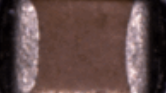
\includegraphics[width=0.3\textwidth]{img/smtcapacitor-sfocatura.png}& Sfocatura & L’immagine viene sfocata tramite un kernel gaussiano per eliminare le componenti di rumore presenti nell’immagine e rendere il successive step di flood fill capace di evadere dalle variazioni di colore introdotte dal rumore.\\
\hline
\vspace{.5mm}
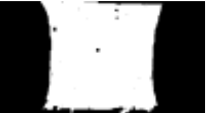
\includegraphics[width=0.3\textwidth]{img/smtcapacitor-ff.png}& Segmentazione del case (FloodFill) & Il case viene rilevato effettuando un flood fill a partire dal baricentro del component ( proveniente dai dati cad). 
Se il risultato del flood fill è un area inferiore a quella attesa
il processo viene ripetuto selezionando casualmente un
punto seme in un intorno del baricentro .\\
\hline
\vspace{.5mm}
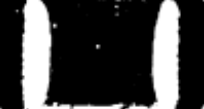
\includegraphics[width=0.3\textwidth]{img/smtcapacitor-pinmask.png}& Pin mask & L’immagine del case è sottrata a quella originale, il risultato di questa operazione viene binarizzato con un metodo di sogliatura alla Otsu.\\
\hline
\vspace{.5mm}

\includegraphics[width=0.3\textwidth]{img/smtcapacitor-pd.png}& Pins detection & L’immagine del case viene ridotta lungo l’asse minore
mediando i valori dei pixel della stessa riga/colonna, l’immagine contenente le intensità risultanti viene sogliata filtrando quindi i picchi non dovuti al pin.\\
\hline
\vspace{.5mm}
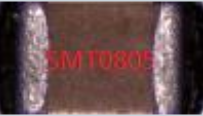
\includegraphics[width=0.3\textwidth]{img/smtcapacitor-measure.png}& Misura & Dalle transizioni nell’immagine output del passo precedente
vengono determinate le larghezze dei pin, dalle transizioni
più lontane viene determinate la larghezza del case,
dall’area ottenuta allo step 2 invece viene determinata
l’altezza del case.
Il risultato del test (score) viene determininato tramite una
metrica di similarità tra il case atteso e quello rilevato, una
mappatura non lineare dei valori viene applicata per
separare meglio score di case simili.
\end{tabularx}

\paragraph{Pattern matching}
Il riconoscimento di pattern è una sottoarea dell'apprendimento automatico. Esso consiste nell'analisi e
identificazione di pattern all'interno di dati grezzi al fine di identificarne la classificazione.
Sui sistemi spea è possibile confrontare l’immagine rilevata dal gruppo ottico con una serie di immagini
campione (acquisite tramite un processo di apprendimento che può essere automatico o supervisionato).


\begin{figure}[!ht]
\centering
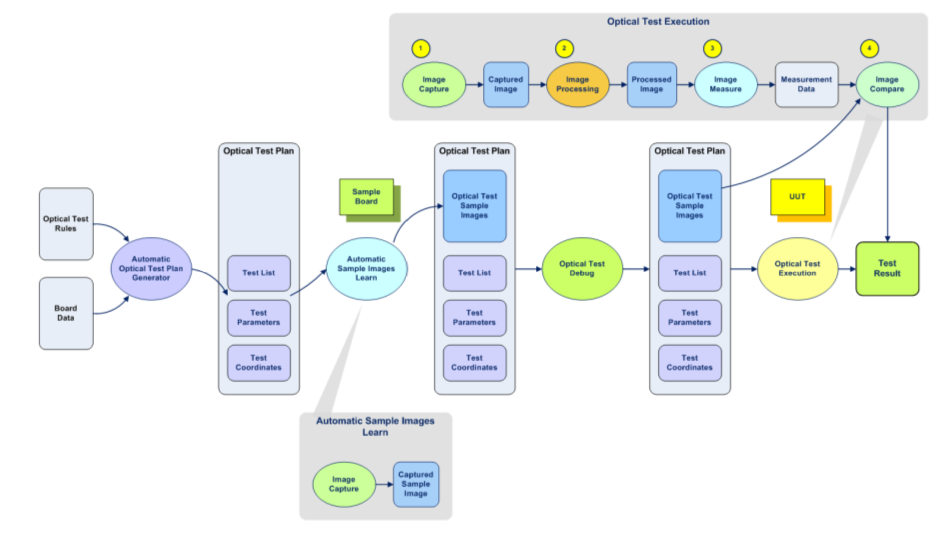
\includegraphics[width=\textwidth]{img/patternmatching.png}
\caption{Flusso di un programma di ispezione ottica tramite pattern matching su flying probe SPEA}
\label{fig:pattern matching}
\end{figure}

\paragraph{Altri utilizzi dell'equipaggiamento di visione}
Un sistema a sonde mobili necessita di precisioni di contattazione bassissime, è per questo che non è
sufficiente inserire un prodotto da testare avendo cura di posizionarlo correttamente.
I sistemi a sonde mobili in ingresso del prodotto effettuano un ispezione ottica per ottenere la
rototraslazione del prodotto rispetto al sistema di riferimento del sistema analizzando la presenza e
soprattutto la posizione di due o più punti fiduciari ( Fiducials ).

\begin{itemize}
\item Il sistema viene acceso, la procedura di homing assicura che il manipolatore cartesiano (dotato di
encoder relativi) trovi lo zero del sistema di riferimento macchina.
\item Una scheda viene caricata in input
\item La sonda dotata di telecamera si posiziona sul punto dove dovrebbe essere localizzato il fiducial.
\item Tramite ispezione ottica automatica viene ricercato tramite template matching un template
precedentemente acquisito e la sua posizione in coordinate immagine viene correlata a quella
dell’asse per ottenere una posizione nel sistema di riferimento macchina
\item Similmente al punto 4 viene ricercato un secondo fiducial sulla scheda da testare.
\item Sono quindi disponibili informazioni sulla rototraslazione della scheda all’interno del sistema e di
conseguenza i successivi spostamenti ( se effettuati nel sistema di coordinate della scheda )
saranno automaticamente corretti. 
\end{itemize}


\subsection{Pick and Place handlers}
\includegraphics[clip=true, trim= 50 260 50 320,page=21,width=0.9\textwidth]{materiale/tesina-carlucci.pdf}

Il test finale è uno dei maggiori processi nella fabricazione dei semiconduttori, risulta necessario testare  i circuiti integrati prodotti prima della consegna al cliente per evitare di propagare fault dei dispositivi prodotti sui prodotti del cliente. 
I flussi di test sono altamente automatizzati ed una fetta importante del mercato dei sistemi di test per 
questa categoria di prodotti è rappresentata da sistemi robotici, i pick and place handler, in grado di 
garantire un elevato throughput. 
I p\&p handler agiscono come meccanismo di trasporto verso le stazioni di test dove il test elettrico viene 
effettuato per poi smistare (binning) i componenti a seconda del risultato del test, motivazione per 
l’utilizzo di sistemi automatici di questo tipo è principalmente la dimensione dei dispositiv i da testare (fino a 2x2 millimetri) che renderebbe difficoltosa la contattazione affidabile se non tramite meccanismi di 
posizionamento ad elevata precisione e la necessità di effettuare il test anche a differenti condizioni di temperatura ( spesso parti per il mercato automotive o militare necessitano di rigidi protocolli di test in 
condizioni avverse). In un contesto di produzione industriale un handler può arrivare a testare fino a 
25000 parti per ora. 

\subsubsection{Composizione di un pick and place handler }

\subsubsection{Dispositivo Di Input }
L’input delle parti da testare può avvenire per mezzo dei meccanismi di caricamento più disparati, i più 
diffusi sono il caricamento per mezzo di vassoi aderenti a standard JEDEC, il caricamento in bobine ed il 
caricamento tramite unità a boccia (bowl feeder) in grado di accettare parti non organizzate in maniera 
specifica e di procedere al sorting su vassoio automatico.  

\subsubsection{Spea Bfu} 

La bowl feeder unit è un dispositivo di input basato su una scodella (bowl) vibrante in grado di caricare i 
componenti sciolti su dei vassoi che successivamente saranno processati dall’unità di handling, l’unità BFU 
è dotata di sistemi di visione necessari a decidere quali movimenti subirà il componente prima di essere 
posato sul vassoio di uscita, due telecamere sono in grado di rilevare su due stazioni diverse del sistema 
di input se il componente è ruotato oppure capovolto e quindi di correggerne l’orientamento inviando 
opportuni segnali di controllo alla stazione contenente l’attuatore.  

\subsubsection{Pick And Place}

L’handling delle parti da testare viene effettuato per mezzo di un manipolatore cartesiano che una volta 
prelevate le parti sotto test dal dispositivo di input procede alla movimentazione lungo il piano orizontale verso le stazioni di test, l’apparato in oggetto è dotato di sonde con pickup di tipo pneumatico in grado di prelevare i componenti senza danneggiarli per mezzo del vuoto, tali sonde sono dotate di 
movimentazione anche lungo l’asse Z.  

\subsubsection{Test Station} 

La test station si occupa di effettuare il test del dispositivo e comunicare al test handler il risultato, essa può essere indipendente dall’handler o strettamente integrata, differenti tipologie di stazioni sono 
disponibili, da notare l’esistenza di stazioni di test elettromeccaniche orientate al collaudo dei mems in 
grado di sottoporli a stimoli meccanici e misure analogiche altamente accurate.  

\subsubsection{Dispositivo Di Output} 

Come per il caricamento l’output può avvenire su una vasta gamma di supporti di uscita, vassoio, bobina, 
tubo. 

\subsection{Spea RSU} 

La reel sort unit è un dispositivo di output in grado di organizzare i componenti in uscita all’interno di 
bobine destinate alla vendita, questa unità è equipaggiata con un sistema di visione in grado di 
riconoscere componenti mal posizionati all’interno della bobina prima di sigillarla, per  tanto effettua un 
test di tasca vuota ed uno di componente ben posizionato. 


\subsection{Tipi di ispezione ottica effettuati da pick and place handlers}
\subsubsection{Calibrazione e built in self test}
Un sistema appartenente alla categoria p\&p handler è in grado di effettuare dei task di calibrazione
riconoscento tramite tecniche di ispezione ottica opportuni punti fiduciari impressi sullo chassis ciò per
mette di evitare derive nel sistema di movimentazione o di verificare tramite riconoscimento di codice a
barre i dispositivi opzionali di natura esclusivamente meccanica necessari a portare a termine la ricetta di
test in uso
\subsubsection{Tracciabilità}
I pick and place handler realizzano spesso funzionalità di tracciabilità riconoscendo per mezzo di
ispezione ottica l’appartenenza di un componente sotto test ad un determinato lotto permettendo la
realizzazione di test cells in grado di effettuare il test di più lotti contemporaneamente e di smistare
correttamente le parti, l’esito di questi controlli può esserere successivamente comunicato al software CIM
dell’industria
\subsubsection{Empty check su tester}
Un componente da testare rimasto bloccato in un sito di test porterebbe ad un falso test poichè
mantenendo la propria contattazione impedendo al nuovo dispositivo di essere contattato porterebbe a
falsi esiti, risulta quindi necessario sviluppare dei test AOI in grado di rilevare la presenza di componenti
bloccati e disabilitare i siti di test per poi informare un operatore.

\endinput